% Nejprve uvedeme tridu dokumentu s volbami
\documentclass[czech,bachelor]{diploma}
% Dalsi doplnujici baliky maker
\usepackage[autostyle=true,czech=quotes]{csquotes} % korektni sazba uvozovek, podpora pro balik biblatex
\usepackage[backend=biber, style=iso-numeric, alldates=iso]{biblatex} % bibliografie
\usepackage{dcolumn} % sloupce tabulky s ciselnymi hodnotami
\usepackage{subfig} % makra pro "podobrazky" a "podtabulky"
\usepackage[cpp]{diplomalst}

% Zadame pozadovane vstupy pro generovani titulnich stran.
\ThesisAuthor{Jakub Pšenčík}

\ThesisSupervisor{Ing. Jan Janoušek}

\CzechThesisTitle{Podpora jazyka Monkey C v prostředí VS Code}

\EnglishThesisTitle{Monkey C Language Support in VS Code}

\SubmissionYear{2021}

% Pokud nechceme nikomu dekovat makro zapoznamkujeme.
\Acknowledgement{Rád bych na tomto místě poděkoval svému vedoucímu práce Ing. Janu Janouškovi za odborné a metodické vedení, ochotu a pomoc v průběhu vypracovávání práce.}

\CzechAbstract{V této bakalářské práci se budu zabývat vývojem rozšíření pro Visual Studio Code, jenž bude poskytovat plnou podporu jazyka Monkey C. Součástí práce bude bude představení prostředí Visual Studio Code a problematika vývoje rozšíření v tomto prostředí. Představen bude, mimo jiné, také jazyk Monkey C. V další části práce se budu zabývat nástrojem ANTLR, díky kterému jsme schopni generovat vlastní překladač jazyka pomocí bezkontextové gramatiky, parsováním kódu a jeho syntaktickou analýzou. Závěrem bude výsledné rozšíření testováno.}

\CzechKeywords{bakalářská práce, rozšíření, Monkey C, Typescript, parser}

\EnglishAbstract{In this bachelor thesis I will deal with the development of extension for Visual Sstudio Code, which will provide full support for Monkey C language. The work will include an introduction to the Visual Studio Code environment and the development of extensions in this environment. Among other things, the Monkey C language will be introduced. In the next part of the work I will describe the ANTLR tool, used to generate our own language compiler using context-free grammar, code parsing and its syntactic analysis. Finally, the resulting extension will be tested.}

\EnglishKeywords{bachelor thesis, extension, Monkey C, Typescript, parser}

\AddAcronym{ANTLR}{ANother Tool for Language Recognition}
\AddAcronym{AST}{Abstract syntax tree}
\AddAcronym{VS Code}{Visual Studio Code}
\AddAcronym{API}{Application Programming Interface}

% odkaz na literaturu
\addbibresource{Citace.bib}

% Novy druh tabulkoveho sloupce, ve kterem jsou cisla zarovnana podle desetinne carky
\newcolumntype{d}[1]{D{,}{,}{#1}}

% Zacatek dokumentu
\begin{document}

% Nechame vysazet titulni strany.
\MakeTitlePages

% Jsou v praci obrazky? Pokud ano vysazime jejich seznam a odstrankujeme.
% Pokud ne smazeme nasledujici dve makra.
\listoffigures
\clearpage

% Jsou v praci tabulky? Pokud ano vysazime jejich seznam a odstrankujeme.
% Pokud ne smazeme nasledujici dve makra.
\listoftables
\clearpage

% A nasleduje text zaverecne prace.
\chapter{Úvod}
\label{sec:Introduction}
V dnešní době, kdy jsme obklopeni spoustou moderních technologií, existující programovací jazyky se stále vyvíjejí kupředu a nové postupně vznikají, existuje nespočet nástrojů, rozšíření, vývojových prostředí, které práci a vývoj na těchto jazycích dokážou v mnoha ohledech usnadnit. Jazyk MonkeyC, jenž bude středobodem této práce, zatím nedisponuje tak široce obsáhlou komunitou, jako mají např. v dněšní době velmi populární Javascript, Python, C Sharp, Ruby, atd...\\

Typickým příkladem společnosti, která se zabývá právě vývojem softwarů pro programátory či vývojáře, je česká JetBrains s.r.o. Ti mají na kontě již mnoho produktů usnadňujících programování, např. ReSharper (.NET), IntelliJ IDEA (Java, Groovy, atd...) či PyCharm (Python). Ovšem na podporu Monkey C zatím žádné softwarové řešení v JetBrains do světa nevypustili. \cite{jetbrains} \\

Na oficiálním webu \cite{marketplace} sice najdeme několik nástrojů, které s vývojem v Monkey C pomáhají, my ale budeme chtít, aby naše aplikace poskytovala co největší podporu uživateli a hlavně, aby byla postavené na našem vlastním řešení.\\

V následujících kapitolách se tedy budeme věnovat tvorbě a vývoji rozšíření pro vývojové prostředí Visual Studio Code, které poskytne plnou podporu při vývoji aplikací. Jako první si představíme jazyk Monkey C, jak se s ním pracuje, jaké aplikace s ním můžeme vyvíjet atd... Pro tvorbu aplikace využijeme jazyk Typescript, dále pak nástroj ANTLR, který se schopný vygenerovat předladač jazyka z jeho popisu obsaženého v bezkontextové gramatice. Další část práce bude věnováná tématům, jako jsou parsování kódu, vytvoření syntaktického a sémantického stromu, našeptávání kódu, atd...
%Jedná se o dynamicky postavený jazyk, stejně jako např. python, R, atd… Jazyk se používá k vývoji aplikací pro Garmin zařízení.\\ V další kapitolách budou detailně popsány klíčové komponenty k vytvoření finální aplikace, např. gramatika pro popis jazyka, ANTLR parser, atd... 
\endinput
\chapter{Jazyk Monkey C}
Monkey C \cite{monkeyc_2021} je objektově orientovaný jazyk navržený pro snadný vývoj Connect IQ aplikací. Jedná se o dynamický programovací jazyk, podobně jako Java, PHP či Ruby. Cílem Monkey C je zjednodušit proces vytváření samotné aplikace a umožnit tak vývojářům více se soustředit na zákazníka a méně na omezení zdrojů. Využívá tzv. "reference counting" k automatickému čištění paměti, což vývojáře osvobozuje od manuální správy paměti (např. jako v jazyce C/C++).
\\
\begin{figure}
	\centering
	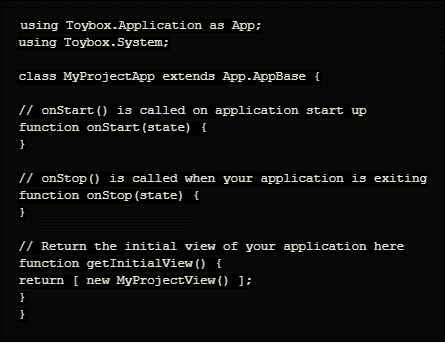
\includegraphics{images/code_snippet}
	\\
	\caption{ukázka jednoduchého fragmentu kódu v MonkeyC}
	\label{img:monkeyC_Fragment}
\end{figure}

\endinput
\chapter{Problematika vývoje rozšíření pro VS Code}

\section{Visual Studio Code}
Visual Studio Code \cite{VSCODE_2020} je editor zdrojového kódu vytvořený společností Microsoft pro operační Windows, Linux a MacOS. Nabízí spoustu užitečných funkcí, mezi které patří podpora ladění kodu, zvýrazňování syntaxe, automatické doplňování a našeptávání kódu, atd… Naším cílem je integrovat většinu těchto funkcí a možností do finálního rozšíření.

\section{Typescript}
TypeScript \cite{TypeScript_wikipedia_2020} je open-source programovací jazyk vyvinutý společností Microsoft. Jedná se o nádstavbu nad jazykem JavaScript,
která jej rozšiřuje o statické typování a další atributy, které známe z objektově orientovaného programování jako jsou třídy, moduly a další. Samotný kód psaný v jazyce TypeScript se kompiluje
do jazyka JavaScript. Jelikož je tento jazyk nádstavbou nad JavaScriptem, je každý JavaScript kód automaticky validním TypeScript kódem.

\section{Komponenty potřebné pro vytvoření rozšíření}
Předtím, než začneme pracovat na samotném rozšíření, je potřeba obstarat několik důležitých nastrojů a komponent, jenž jsou klíčové při vývoji.
\subsection{Gramatika}
Jako první je potřeba definovat popis jazyka MonkeyC. V našem případě je jazyk popsán prostřednictvím bezkontextové gramatiky, která formálně definuje syntax (pravidla) jazyka.

\begin{figure}
	\centering
	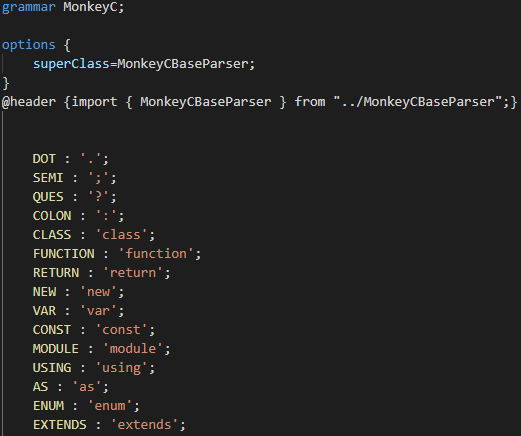
\includegraphics[scale=0.8]{images/grammar}
	\caption{ukázka hlavičky gramatiky MonkeyC.g4 pro popis jazyka}
	\label{img:grammar}
\end{figure}

Na obrázku mužeme vidět prvních pár řádků gramatiky pro MonkeyC. Gramatika obsahuje spoustu známých klíčových slov, nebo-li tokenů, např. "CLASS", "FUNCTION", "USING", atd...

\subsection{Java}
Jelikož je ANTLR psán v Javě, je potřeba ji nainstalovat na naše zařízení, přičemž se požaduje verze 1.6 nebo vyšší. Poté již stačí stáhnout akualní ANTLR jar, což je momentálně "antlr-4.8-complete.jar".

\subsection{Parser a Lexer}
\textbf{lexer} - lexer (nebo také tokinizér) "rozdělí" text na vstupu (v našem případě MonkeyC kód) na tokeny. \cite{ANTLR_PG_20} \\
\textbf{parser} - shora dolů prochází text na vstupu a porovnává jednotlivé řádky s pravidly obsažené v gramatice.\\
K vytvoření parseru a lexeru je potřeba spustit ANLTR nástroj, který s pomocí gramatiky tyto souboru vygeneruje. \cite{ANTLR_PG_20} \\

\begin{figure}
	\centering
	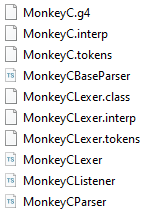
\includegraphics{images/generated_files}
	\\
	\caption{potřebné soubory vygenerované nástrojem ANTLR}
	\label{img:generated_files}
\end{figure}

\subsection{TestRig}
ANTLR poskytuje flexibilní testovací nástroj umístněný v runtime knihovně s názvem TestRig. TestRig dokáže poskytnout spoustu informací o tom, jak "recognizéry" (parser a lexer) zpracovávají InputStream ze vstupního souboru.\\
Nejjednodušší způsob ověření, zda gramatika rozpoznává vstup správně, je zobrazit si vygenerovaný syntaktický strom vizuálně.

\begin{figure}
	\centering
	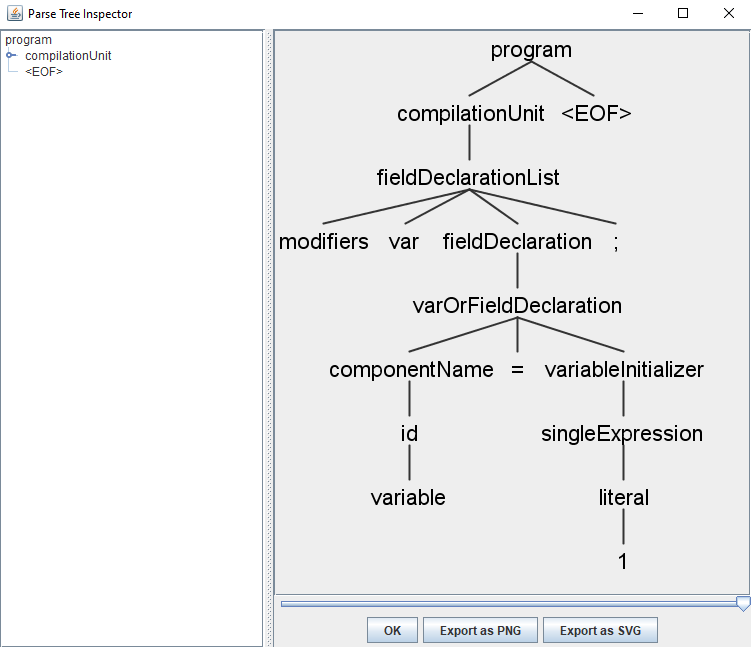
\includegraphics[scale=0.8]{images/ParseTreeInspector}
	\caption{"ParseTreeInspector" - vizuální podoba syntaktického stromu} 
	\label{img:ParseTreeInspector}
\end{figure}
Na obrázku můžeme detailně vidět jak parser vytvořil syntaktický strom a jak jsou jednotlivé části propojené. Strom začíná kořenem, jenž je v naší gramatice pojmenová, jako "program". Takto je kořen pojmenován při každém parsování. 

\endinput
\chapter{Syntaktická a sémantická analýza kódu}
Abychom mohli implementovat náš jazyk (MonkeyC), je potřeba vytvořit aplikaci, která je schopna číst "věty" na vstupu a odpovídajicím způsobem rozpoznává klíčová slova či fráze naší gramatiky.(Obecně je jazyk složení platných vět, kdy věta se skládá z frází a fráze se skládá ze symbolů slovní zásoby).\\
Obecně lze říci, pokud nějaká aplikace vykonává (interpretuje) zápis jiného programu v jeho zdrojovém kódu ve zvoleném programovacím jazyce (v našem případě Typescript), že se jedná o tzv. interpret \cite{Interpret_2020}. Jako příklady je možné uvést kalkulačku, aplikace pro čtení konfiguračních souborů, Python interprety, atd... Pokud, na druhou stranu, dochází k převodu "věty" z jednoho jazyka do druhého (např. z Javy do 'C Sharp'), nazývá se taková aplikace překladačem.\\
Úkolem překladače či interpreta je tedy rozpoznat platné vstupy, tedy věty, fráze, subfráze, klíčová slova, atd... Přičemž rozpoznáním platného vstupu je myšleno identifikovat jednotlivé fráze a rozližit je od jiných.\\
Jako příklad použijeme rozpoznání vstupu $input = 1;$ s validní MonkeyC syntaxí. Syntaktický strom z těchto vstupních dat je možné vidět na obrázku \ref{img:assigment}. Z tohoto vstupu je patrné, že "input" je cíl přiřazení a "1" představuje hodnotu, která se má přiřadit. Stejně jako jsme my schopni rozližit v našem jazyce sloveso od podstatného jména, je naše aplikace schopna rozlišit toto přiřazení od např. importování knihovny pomocí klíčového slova "using".\\
Programy, které jsou schopny rozpoznávat konkrétní jazyk, se nazývají parsery nebo syntaktické analyzátory, přičemž syntax odkazuje na pravidla obsažená v popisu jazyka.\\

\begin{figure}[b!]
	\centering
	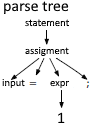
\includegraphics[scale=1.5]{images/assigment}
	 \caption{přiřazení hodnoty 1 proměnné input}
	 \label{img:assigment}
\end{figure}


\section{Parser a Lexer}
K vytvoření parseru a lexeru je potřeba spustit ANLTR nástroj, který na základě popisu jazyka (gramatiky) tyto souboru vygeneruje. S jejich pomocí je poté možné generovat syntaktické stromy pro vstupní data. Zde platí, že pokud jsou vstupní data validní (nejsou v rozporu s pravidly gramatiky), tak je vygenerovaný parser vždy rozpozná správně nehledě na složitost gramatiky.\\
Proces, při kterém dochází ke skládání znaků ze vstupních dat do slov či symbolů (tokenů) nese název \textbf{lexikální analýza} nebo \textbf{tokenizace}. Program, který provádí tuto tokenizaci se nazývá právě \textbf{lexer}. Obecně lze říci, že lexer (nebo také tokenizér) "rozdělí" text na vstupu (Monkey C kód) na tokeny. \cite{ANTLR_PG_20}. Dále lexer dokáže vytvořené tokeny seskupovat do tokenových tříd, nebo typů, např. IDENTIFIER (identifikátor), INTLITERAL (celočíselná proměnná), DOUBLELITERAL (proměnná typu double), atd...
V momentě, kdy lexer rozdělil vstupní data na jednotlivé tokeny, jsou tyto tokeny předány parseru. Ten poté "shora dolů" prochází text na vstupu a porovnává jednotlivé řádky s pravidly obsažené v gramatice \cite{ANTLR_PG_20}. Na obrázku \ref{img:parser} je možné vidět, jak parser zpracovává vstup $sp = 100;$. Tokeny, které lexer z těchto dat rozpozná, jsou [SP, =, 100, ;, <EOF>], kde SP je název proměnné, 100 hodnota, která je proměnné přiřazena, jako ve většině programovacích jazyků musí být příkaz ukončen středníkem, <EOF>, který se vyskytuje na konci každého validního vstupu, detekuje konec souboru (EOF - End Of File).


\begin{figure}[b!]
	\centering
	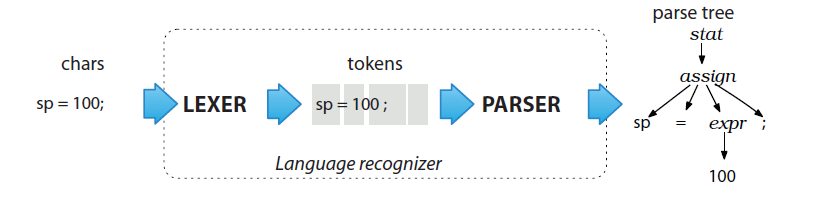
\includegraphics[scale=0.7]{images/parser}
	\caption{Ukázka, jak Language recognizer zpracovává vstupní sekvenci znaků} 			    \cite{ANTLR_PG_10}
	\label{img:parser}
\end{figure}

\section{Syntaktický strom}
Syntaktický strom představuje datovou strukturu, kterou ANTLR vytvoří při parsování vstupního souboru. Struktura je složená z kořene (root) a uzlů, které mohou představovat buď další podstromy, které odpovídají pravidlům gramatiky, nebo listy stromu.\\ 
V naší aplikaci Syntaktický strom představuje třída AST \ref{code:Node_TS}, která uchovává všechna důležitá data pro korektní analýzu vstupního souboru, např. počet uzlů stromu, soubor vztahující se ke konkrétnímu stromu, kořen stromu, atd...

\lstinputlisting[label=code:AST_TS,caption={třída AST v jazyce Typescript}]{SourceCodes/AST.tss}

Další, neméně důležitou, třídou v naší apikaci je třída Node, která představuje uzel stromu. Jedná se, ve své podstatě, o strukturu uchovávající následující atributy:\\
\begin{enumerate}
	\item kontext daného uzlu
	\item předka uzlu
	\item potomka uzlu
	\item hodnotu přestavující text daného uzlu
	\item typ uzlu, který se odvíjí od pravidel v gramatice
\end{enumerate}

\lstinputlisting[label=code:Node_TS,caption={třída Node v jazyce Typescript}]{SourceCodes/Node.tss}


\section{ANTLR Listener a callback funkce}
ANTLR disponuje dvěma mechanismy, které umožňují průchod stromem (tzv. "tree-walking mechanisms"). Jedná se o mechanismy \textbf{listener} a \textbf{visitor},pričemž výchozím je listener. Největší rozdíl mezi nimi spočívá v tom, že listener metody jsou volány nezávisle ANTLR objektem, zatímco visitor metody vyvolávají rovněž metody potomků uzlu, na kterém se právě nachází, což způsobuje, že některé podstomy nebudou při průchodu vůbec navštíveny. Samotné listenery jsou ekvivalentí SAX objektům, které se používají v XML parserech.\\
Aby bylo možné stromem procházet a při průchodu vyvolat odpovídající události, ANTLR dispinuje třídou ParseTreeWalker. Právě ona se stará o to, aby byly volány callback funkce. Další důležitou komponentou, vygenerovanou ANTLR nástrojem je rozhraní ParseTreeListener (v našem případě MonkeyCListener \ref{img:generated_files}). Toto rozhraní definuje veškeré metody potřebné k kompletnímu průchodu stromem, např. "enterFunctionDeclaration(context: FunctionDeclarationContext)" či "exitFormalParameterDeclarations(context: FormalParameterDeclarationsContext)" \ref{img:listener_functions}. 

\begin{figure}[tbh!]
	\centering
	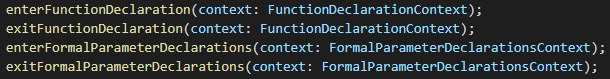
\includegraphics[scale=1]{images/listener_functions}
	\caption{funkce vygenerované nástrojem ANTLR} 			    
	\label{img:listener_functions}
\end{figure}

Ke každému pravidlu obsaženému v gramatice, parser vygeneruje 2 metody a kontextovou třídu. První metoda vždy začíná prefixem "enter" a druhá prefixem "exit", kontext poté odpovídá příslušnému pravidlu. Ve chvíli kdy ParseTreeWalker narazí na příslušný uzel, vyvolá odpovídající metodu, podle toho zda do uzlu vstupuje, nebo jej opouští.


\section{Sémantická analýza} \label{44SemantickaAnalyza}

Sémantická analýza, ve většině případů, spočívá v nalezení a uložení všech identifikátorů vyskytujících se ve zdrojovém kódu programu. Identifikátory jsou myšleny proměnné, konstanty, funkce, atd... Při analýzy jsou dále vyhledávány informace o jednotlivých identifikátorech, např. datový typ proměnné, zda-li již byla deklarována, zda je správně použita vzhledem k jejímu datovému typu, atd... Pro uložení všech těchto informací se, opět ve většině případů, používá tabulka symbolů. Na obrázku \ref{img:tabulka_symbolu} lze vidět, jak taková tabulka symbolů může vypadat. Tabulka o každé proměnné uchovává její název, velikost v Bytech, zda již byla v programu deklarována a použita.\\

\begin{figure}[b!]
	\centering
	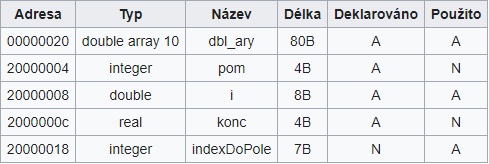
\includegraphics[scale=0.8]{images/symbol_table}
	\caption{ukázka tabulky symbolů \cite{tabulka_symbolu}} 			    
	\label{img:tabulka_symbolu}
\end{figure}

Tabulka symbolů působí jako velmi efektivní nástroj pro sémantickou analýzu. Dokáže uchovávat všechny identifikátory v kódu a informace o nich. V této práci však tabulka symbolů použita není. Hlavním důvodem byla nedostatečná znalost této problematiky na začátku tvorby práce.\\
Sémantická analýza je v této práci řešena ve třídě documentHandler.ts, která je detailněji popsána v další kapitole. Pro uchovávání informací o identifikátorech v kódu jsou použity Mapy. Typescript Mapa představuje datovou strukturu, která byla nově představena v ECMAScriptu 6 \cite{ES6}. Mapa dokáže ukládat data ve formátu klíč - hodnota, stejně jako Mapy v ostatních programovacích jazycích, např. Java, C Sharp.\\
Mapy, které rozšíření používá jsou následující: \begin{enumerate}

\item \textbf{diagnosticMap : Map<string, vscode.DiagnosticCollection>} - Mapa, která pro každý dokument uchovává chyby ve zdrojovém kódu programu. Pro detekování těchto chyb je použita třída ErrorListener.ts (popsána v kapitole 5).

\item \textbf{documentAutocompleteMap : Map<string, Map<string, vscode.CompletionList>>} - Mapa, ve které jsou uloženy všechny proměnné, funkce, konstanty. Tyto data poté rozšíření našeptává podle toho, jaký provider je zrovna spuštěn (pozn. provider jsou popsány v kapitole 5). Klíčem pro tuto mapu je název dokumentu, ke kterému se vztahuje. Hodnotou je opět Mapa, jejíž klíčem je druh identifikátoru (např. \textbf{localVariables} - pro lokální proměnná, \textbf{functions} - pro funkce) a hodnotou je seznam těchto identifikáturů (tedy např. seznam proměnných, seznam funkcí,...). 

\item \textbf{abstractSyntaxTreeMap : Map<string, AST | any>} - Mapa, která pro každý dokument uchovává jeho syntaktický strom vygenerovaný ANTLR nástrojem. Hodnotou je název příslušného dokumentu, hodnotou pak instance třídy AST \ref{code:AST_TS}. Tato mapa je zde zařazena, jelikož vyhledávání v syntaktickém stromě je rovněž součástí sémantické analýzy.

\item \textbf{abstractSyntaxTreeCommentaryMap : Map<string, Token[] | any>} - Mapa, ve které jsou uloženy všechny komentáře z daného dokumentu. Nástroj ANTLR při generování syntaktického stromu totiž neukládá samotný kód a jeho komentáře společně. Kód a komentáře jsou rozděleny do kanálů, přičemž kód je uložen v kanálu s indexem 0, a komentáře jsou uloženy v kanálu 1. Bylo proto nutné vytvořit 2 mapy, jednu pro syntaktický strom, a druhou pro komentáře. Význam a využití komentářů v rozšíření je vysvětlena v další kapitole.
\end{enumerate}

\endinput

\chapter{Návrh a implementace rozšíření}
Rozšíření bude implementováno v jazyce Typescript. K vytvoření rozšíření samotného je potřeba Node.js \cite{nodejs} a Git \cite{git}. Poté je vyžadována instalace programů Yeoman \cite{yeoman} a VS Code Extension Generator \cite{YO_Generator}, pomocí kterých jsou rozšíření generovány.\\

\section{Třída extension.ts}
Základní třída, která je součástí každého VS Code rozšíření, je třída \textbf{extension.ts}. Na začátku třída obsahuje pouze jedinou funkci, a to \textit{function activate(context: vscode.ExtensionContext)}. Tato Funkce rozšíření aktivuje, pokud narazí na soubor s příponou \textbf{.mc}. Seznam přípon souborů, při jejich otevření se rozšíření aktivuje, je uveden v konfiguračním package.json souboru, viz \ref{src:activation}. Rozšíření se také aktivuje v případě, že pracovní adresář obsahuje Monkey C soubor. V package.json souboru jsou mimo jiné uvedeny informace, jako název rozšíření, jeho popis, autor, aktuální verze, atd...\\

\begin{lstlisting}[language=Python,label=src:activation,caption={aktivační události rozšíření}]
        "activationEvents": [
			"onLanguage:monkeyc",
			"workspaceContains:.mc"
		]
\end{lstlisting}

Funkce \textit{\textbf{activate()}} přijímá parametr context. Tento parametr reprezentuje nástroje, se kterými rozšíření pracuje. Tělo funkce se skládá z několika podpůrných tříd, tzv. providerů. Providery jsou součástí VS Code API (jedná se o sadu JavaScript rozhraní, které mohou být vyvolány rozšířením) \cite{vscodeAPI}. \\
První provider ve třídě extension zajišťuje obarvování Monkey C syntaxe, viz. \ref{sec:obarveni_kodu}. Dále následuje funkce \textit{onDidOpenTextDocument()}. Jedná se o událost, která se vyvolá při otevření textového dokumentu. Zde je také řešeno parsování souborů. Pokud uživatel otevře pracovní adresář, tedy složku, která obsahuje více soborů, spustí se funkce parseAllDocuments(). Událost \textit{onDidChangeTextDocument()} společně s funkcí parseCurrentDocument() dále řeší parsování aktuálně upravovaného dokumentu, a to vždy když dojde k nějaké změně. Dále třída extension.ts obsahuje sadu providerů, které zajišťují našeptávání a dokončování kódu \ref{src:completionProvider}. Tento provider přijímá následující tři parametry: 

\begin{enumerate}
\item \textbf{selector} - definuje dokumenty, na které má být provider aplikován
\item \textbf{provider} - definuje konkrétní provider
\item \textbf{...triggerCharacters} - jedná se o pole znaků, při kterých má být provider aktivován. V rozšíření jsou pro aktivaci providerů nejčastěji použity symboly tečky a mezery
\end{enumerate}

\textbf{keywordsProvider} - Provider zajišťující našeptávání klíčových slov jazyka. Pro získání vhodných klíčových slov je použit c3 Engine, popsán v sekci \ref{55section}\\

\textbf{importedModulesProvider} - Pokud jsou ve zdrojovém kódu programu, prostřednictvím klíčového slova \textbf{using}, importovány nějaké moduly, tento provider vrátí jejich seznam. V následujícím výpisu kódu je importováno 5 modulů a 1 třída z Toyboxu. Seznam který provider vrátí bude tedy obsahovat 5 názvů modulů a 1 název třídy [WatchUi, Graphics, System, Lang, Object, Time], kde Object je název třídy. V tomto seznamu jsou hodnoty uloženy jako \textbf{vscode.CompletionItem} \ref{img:CompletionItem}. Jedná se o třídu, která je součástí VS Code API. Její konstruktor přijímá 2 parametry, název položky a její druh. Druh položky, CompletionItemKind, představuje výčet, který obsahuje prvky, jako modul, třída, proměnná, funkce, konstanta, atd...\\


\begin{lstlisting}[language=Python,label=src:usingStatements,caption={importované moduly z Toyboxu}]
      using Toybox.WatchUi;
		using Toybox.Graphics;
		using Toybox.System;
		using Toybox.Lang;
		using Toybox.Lang.Object;
		using Toybox.Time;
\end{lstlisting}



\begin{lstlisting}[language=Python,label=src:completionProvider,caption={aktivační události rozšíření}]
        registerCompletionItemProvider(selector: DocumentSelector, provider: CompletionItemProvider, ...triggerCharacters: string[]): Disposable
\end{lstlisting}

\textbf{localVariableProvider} , \textbf{classVariableProvider} -Providery zajišťující našeptávání lokálních proměnných ve zdrojovém kódu. V Monkey C existují 2 způsoby, jak lze přistupovat k proměnným. Pokud se jedná o vnitřní proměnnou třídy, přístup k ní není nijak omezen. Pokud je proměnná označena jako \textbf{public} nebo \textbf{protected}, je potřeba k ní přistoupit pomocí prefixů \textbf{self.} nebo \textbf{me.}.\\

\begin{figure}
	\centering
	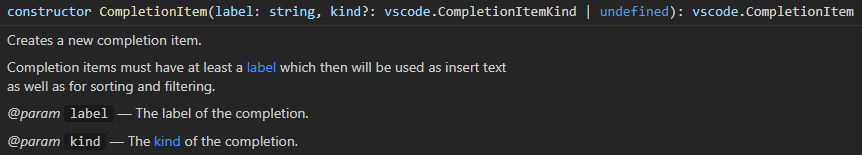
\includegraphics[width=\textwidth,scale=1]{images/CompletionItem}
	\caption{popis konstruktoru třídy CompletionItem z VS Code API}
	\label{img:CompletionItem}
\end{figure}

\textbf{functionProvider} - Provider pro funkce ve zdrojovém kódu. Výše bylo zmíněno, že každá funkce musí být před použitím deklarována a nelze ji předat přímo, jako parametr jiné funkci. Pokud však použijeme funkci \textbf{method()} z třídy Toybox.Lang.Object, instance této třídy dokáže vytvořit objekt třídy Toybox.Lang.Method, díky které je tuto funkci vyvolat, jako callback, viz. výpis kódu \ref{src:callback}.\\

\textbf{toyboxProvider} - slouží pro našeptávání komponent Toyboxu při importování do aplikace, např. modulů a tříd, viz. výpis kódu \ref{src:usingStatements}. Pro získání modulů je použita funkce \textit{findModuleBodyMembers()}, která prochází syntaktickém strom a hledá uzel, ve kterém je uložen Toybox. Jelikož je tento modul rodičem pro všechny ostatní moduly, stačí nalézt první uzel, který obsahuje pravidlo \textit{$MonkeyCParser.RULE_moduleBodyMembers$}, viz. výpis kódu \ref{src:findModuleBodyMembers}. Následně stačí pomocí metody \textbf{getChildren()} získat všechny jeho potomky. Z těchto potomků poté funkce \textbf{collectClassesFromModules()} získá názvy všech tříd, které je možné importovat.\\

\begin{lstlisting}[language=Python,label=src:callback,caption={ukázka použití funkce, jako callback}]
    //! Constructor
    function initialize()
    {
        View.initialize();
        Sensor.enableSensorEvents( method(:onSnsr) );

    }

    function onSnsr(sensor_info)
    {
        //function body
    }
\end{lstlisting}

\begin{lstlisting}[language=Python,label=src:findModuleBodyMembers,caption={funkce prochází strom a hledá uzel, ve kterém je uložen Toybox}]
                    if(tree[i].getContext()!?.ruleIndex === MonkeyCParser.RULE_moduleBodyMembers) {
                    modules = tree[i].getChildren()!;
                    break;
                }
\end{lstlisting}

\textbf{accessibleMembersProvider} - Tento provider zajišťuje především našeptávání na proměnných nějakého typu, jak je možné vidět na obrázku \ref{img:autocomplete_example}, kde rozšíření našeptává metody z třídy Toybox.Lang.String. Pokud je tedy proměnná například instance třídy, nebo se jedná o importovaný modul, provider podle toho v syntaktickém stromě nalezne, co se pod daným identifikátorem nachází, a podle toho jsou volány příslušné funkce. Například pro nalezení všech přístupných členů instance třídy je použita funkce \textbf{collectAccessibleMembers()}.\\

\textbf{inheritedMembersProvider} - Jsou deklarovány třídy \textbf{A} a \textbf{B}, kde třída \textbf{B} je potomkem třídy \textbf{A}. V Monkey C je dědičnost podporována a k její identifikaci je použito klíčové slovo \textbf{extends}. V tomto případě by tedy deklarace třídy B vypadala \textit{class B extends A {}}. Pokud chceme přistoupit ke členům rodičovské třídy A, provede tento provider příslušné operace a vrátí seznam dostupných členů.\\

\textbf{importedMembersProvider} - Tento provider se stará o našeptávání tříd z importovaných modulů. Na obrázku \ref{img:importedModules} lze vidět, jak rozšíření našeptává prvních 5 tříd z importovaného modulu Toybox.Application. Provider je aktivován, pokud se na řádku nachází klíčové slovo \textbf{new}, tím pádem pozná, že chce uživatel vytvořit novou instanci třídy.\\


\begin{figure}[b!]
	\centering
	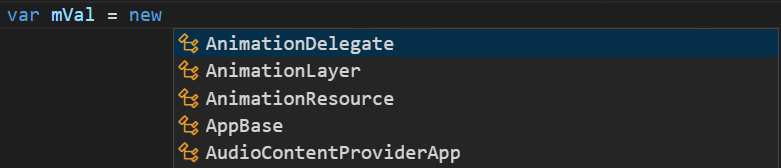
\includegraphics[width=\textwidth,scale=1]{images/importedModules}
	\caption{rozšíření našeptává třídy z importovaných modulů.}
	\label{img:importedModules}
\end{figure}

\textbf{curlyBracesProvider}, \textbf{normalBracesProvider} - Zde bylo záměrem automaticky do dokumentu doplnit pravou závorku po zadání levé. Například v situaci, kdy uživatel napíše levou závorku '\textbf{$($}', rozšíření automaticky do textu doplní druhou. Doplnit takto závorku do dokumentu se však nepodařilo. Místo toho provider uživateli závorku navrhne, stejně jako navrhují kandidáty ostatní providery, a ten ji následně po stisknutí tlačítka tab na klávesnici doplní.\\

\textbf{multilineCommentProvider} - Tento provider zajišťuje našeptávání 2 typů víceřádkových komentářů. První typ je klasický prázdný víceřádkový komentář, který nalezneme ve většině programovacích jazyků. Druhý typ, který je možné vidět na obrázku \ref{img:comments}, je specifický tím, že v sobě obsahuje \textbf{@type}. Tento komentář slouží k popisu proměnné při její deklaraci. Za prefix  \textbf{@type} uživatel uvede datový typ proměnné. Je zde využito toho, že v Monkey C musí být proměnná před použitím deklarována, jak už zde bylo několikrát zmíněno a jak je popsáno v sekci \ref{55section}.\\

\textbf{dataTypesProvider} - Další a zároveň poslední provider ve třídě \textbf{extension.ts}, který úzce souvisí s providerem předchozím, je dataTypesProvider. Jak už je z názvu patrné, provider zajišťuje našeptávání všech datových typů z Toyboxu. Na obrázku \ref{img:data_types} lze vidět, jak rozšíření našeptává datové typy z Toyboxu.\\

\begin{figure}[h!]
	\centering
	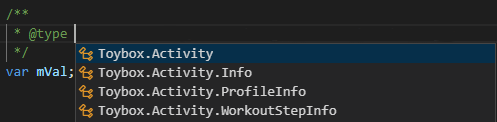
\includegraphics[width=\textwidth,scale=1]{images/data_types}
	\caption{rozšíření našeptává datové typy z modulu Toybox.Activity.}
	\label{img:data_types}
\end{figure}

Na začátku této sekce byla zmíněna funkce \textit{activate()}, která je volána při spuštění rozšíření. K ní je, jako protiklad, na konci funkce \textit{deactivate()}, která je volána v momentě, kdy je deaktivováno rozšíření.\\

\section{Třída documentHandler.ts}
Jedná se o jednu z nejdůležitějších a nejrozsáhlejších tříd v celé aplikaci. Obsahuje přes 30 metod, které zajišťují plynulý chod rozšíření. Nacházejí se zde Mapy, ve kterých jsou uloženy veškeré informace jednotlivých dokumentů, jak je popsáno v sekci \ref{44SemantickaAnalyza}. Nejdůležitějšími třídami jsou však \textit{\textbf{parseAllDocuments()}} a \textit{\textbf{parseCurrentDocument()}}. Funkce \textit{\textbf{parseAllDocuments()}} je při aktivaci rozšíření volána jako první. Zde dochází k načtení všech souborů z pracovního adresáře. Následně je pro daný soubor vytvořen \textit{inputStream}, jenž je jako parametr předán instanci \textbf{MonkeyCLexer}u. Dále dojde k vytvoření \textbf{tokenStream}u, jenž je předán instanci \textbf{MonkeyCParser}u. Poté dojde k parsování dokumentu a vytvoření syntaktického stromu jak pro zdrojový kód, tak pro komentáře, viz. obrázek \ref{img:parsing_input}.\\


\begin{figure}[]
	\centering
	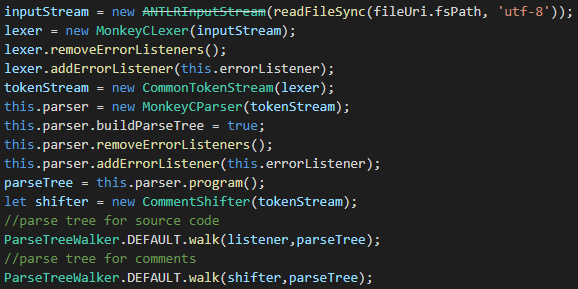
\includegraphics[width=\textwidth,scale=1]{images/parsing_input}
	\caption{vytvoření instancí parseru a lexeru a následné parsování soboru.}
	\label{img:parsing_input}
\end{figure}

Dále je volána funkce \textbf{provideAutocomplete()}, která ze syntaktické stromu získá proměnné, funkce, atd... Vždy pro konkrétní dokument. Funkce updateCollection() poté zpracuje všechny syntaktické chyby, která detekoval Error Listener \ref{errorListener}.\\

Funkce \textit{\textbf{parseCurrentDocument()}} vykonává stejnou činnost, jako výše popsaná pouze s tím rozdílem, že tato funkce je volána vždy při práci s konkrétním dokumentem.

\section{Třída Listener.ts}
Jedná se o třídu, která implentuje rozhraní \textbf{MonkeyCListener}. Toto rozhraní  definuje kompletní listener pro parser vytvořený \textbf{MonkeyCParser}em. jinými slovy, nacházejí se zde všechny metody, které jsou potřeba pro vytvoření syntaktického stromu při průchodu parseru. Příklad vytvořených metod je možné vidět na obrázku \ref{img:listener_functions}. Kromě zpracovávání zdrojového kódu třída Listener zajišťuje také zpracování komentářů. Toto je zajištěno prostřednictvím třídy \textit{CommentShifter}, převzaté z Definitive ANTLR 4 reference \cite{ANTLR_2013}. Tato třída umožňuje přístup ke skrytému kanálu s komentáři, které jsou od zdrojového kódu odděleny.

\section{Error Listener} \label{errorListener}
Třída, která slouží k detekování zachytávání syntaktických chyb v kódu. Jedná se o chyby, které jsou v rozporu z pravidly gramatiky. Každá chyba, kterou rozšíření detekuje, je uložena do struktury \textbf{ErrorDescription} \ref{src:ErrorDescription}. Všechny chyby jsou poté uloženy v poli a pomocí metody getSyntaxErrors() je možné je získat. Rozšíření chyby vypisuje do konzole, jak je ve VS Code zvykem. Součástí zprávy jsou:
\begin{enumerate}
\item řádek, na kterém se chyba nachází
\item pozice na řádku
\item popis chyby
\end{enumerate}

\begin{lstlisting}[language=Python,label=src:ErrorDescription,caption={rozhraní pro popis chyby}]
export interface ErrorDescription {
	document: string;
	offendingSymbol: any;
	line: number;
	charPositionInLine: number;
	msg : string
	e: RecognitionException | undefined
}
\end{lstlisting}

\section{Modul Toybox}
Modul Toybox představuje v Monkey C jmenný prostor (namespace), pod kterým jsou seskupovat třídy, metody, funkce, atd... Obsahuje všechny potřebné třídy, které Monkey C poskytuje, na jednom místě. Z názvů jednotlivých modulů a tříd lze jednoduše odvodit, jaké metody se zde nachází a k jakému účelu slouží.\\ 
Jelikož tento modul, není nikde oficiálně dostupný. Respektive neexistuje žádná oficiální verze, kterou by bylo možné použít, bylo nutné sestavit modul vlastními silami. K jeho vytvoření bylo použito oficiální Connect IQ SDK. V tomto SDK jsou obsaženy informace, ke všem komponentům Toyboxu. Problémem bylo, že zdrojem těchto informací byly soubory ve formátu .html, tedy webové stránky. Bylo tedy nutné veškeré informace extrahovat z html elementů a následně je sestavit do požadované formy. Jelikož bylo vygenerování Toyboxu velmi pracné a extrakce jednotlivých částí z html elementů vyžadovala mnoho úsilí, není zaručeno, že je Toybox zcela kompletní. Vygenerovaný Toybox například neobsahuje deklarované konstanty, které se v některých třídách v oficiální dokumentaci nachází. Velkou výhodou by bylo, kdyby společnost Garmin Ltd. \cite{GARMIN_OFFICIAL} vydala svoji plnohodnotnou verzi Toyboxu. Toto by při vývoji rozšíření ušetřilo velké množství práce a času stráveném při jeho generování.

\section{Obarvení kódu} \label{sec:obarveni_kodu}
Zvýraznění a obarvení Monkey C syntaxe bylo převzato z GitHub repozitáře \cite{syntax_highlight}. Autor Alexander Fedora \cite{fedora} zde k obarvení klíčových slov Monkey C využívá JSON souboru. Tento soubor obsahuje všechna klíčová slova, ty pomocí regulárních výrazů vyhledává v textu a poté je obarvuje.

\begin{figure}
	\centering
	\subfloat[před\label{img:uncolored_code}]
	{
		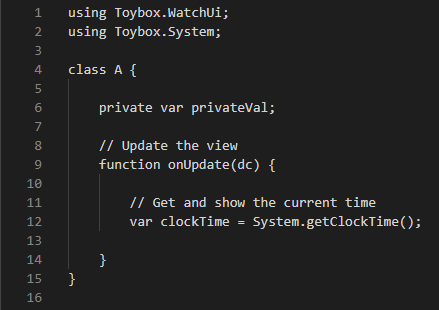
\includegraphics[width=0.45\textwidth]{images/uncolored_code}
	}
	\hspace{1.5em} % make more space
	\subfloat[po\label{img:colored_code}]
	{
		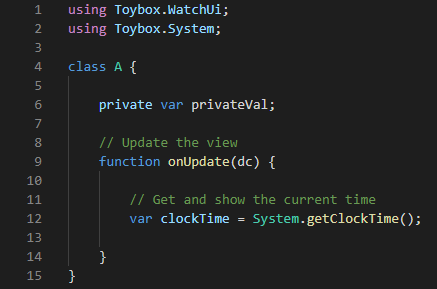
\includegraphics[width=0.45\textwidth]{images/colored_code}
	}
	\caption{Monkey C kód před a po přidaní obarvení syntaxe}
	\label{img:obarveni}
\end{figure}
	
Hned na první pohled je zřejmé, že obarvení poskytuje uživateli větší přehled a orientaci v kódu, jak je vidět na obrázku \ref{img:colored_code}.


\section{Automatické doplňování a našeptávání kódu} \label{55section}
Jako první bylo v rozšíření řešeno našeptávání klíčových slov jazyka, např. NEW, VAR, FUNCTION, atd... k tomuto účelu byl použit "The ANTLR4 Code Completion Core"  \cite{mike_lischke}. Jedná se o "stroj"  sloužící k dokončování kódu pro analyzátory založené na ANTLR4. Engine c3 je schopen poskytnout kandidáty na doplnění kódu, kteří jsou užiteční pro editory s analyzátory generovanými ANTLR, nezávisle na skutečném jazyku / gramatice použité pro generování. Původní implementace je poskytována v jazyce Typescript, což bylo vhodné použít vzhledem k tomu, že rozšíření je také psáno v Typescriptu.
\\
Dále bylo řešeno našeptávání lokálních funkcí a proměnných. V Monkey C jsou k tomuto účelu použity 2 prefixy \textbf{self.} a \textbf{me.}. Pokud uživatel v kódu zadá jeden z těchto prefixů, rozšíření spustí funkci \textbf{provideAutocomplete}, která pomocí průchodu syntaktickým stromem všechny dostupné proměnné, funkce, či třídy, podle toho, kde se zrovna uživatel v kódu nachází.
\\
V neposlední řadě bylo potřeba vyřešit, jak zjistit, co se nachází v konkrétní proměnné, a na základě toho poté provést příslušné našeptávání. Toto je řešeno  pomocí komentářů. Tyto Komentáře se objevují jednak v Toyboxu, kde slouží pro orientaci v už tak rozsáhlém modulu a popisu jednotlivých jeho součástí. Součástí popisu jsou informace o datových typech, vstupních parametrech ( pokud se jedná o funkci), návratových typech atd...  
\\
Komentáře má také k dispozici uživatel přímo v kódu. Každá proměnná, která je deklarována, by měla na sebou obsahovat komentář nesoucí informaci o datovém typu této proměnné. Komentář má jednoduchou syntax, viz. \ref{src:comment}, a rozšíření je navíc schopné jeho stukturu automaticky doplnit po zadání "\textbf{/**}". Je zde využito toho, že každá proměnná v Monkey C musí být deklarována předtím, než ji lze použít. A právě na základě tohoto byly v rozšíření komentáře implementovány. Není tedy potřeba složitě hledat a ukládat informace o datovém typu do nějaké struktury, stačí pouze v kanálu komentářů najít příslušný řádek, na kterém je proměnná deklarována a z něj datový typ extrahovat.

\begin{lstlisting}[language=Python,label=src:comment,caption={struktura komentáře datový typ}]
        /**
         * @type Toybox.Lang.Number
         */
\end{lstlisting}

\begin{figure}[tbh!]
	\centering
	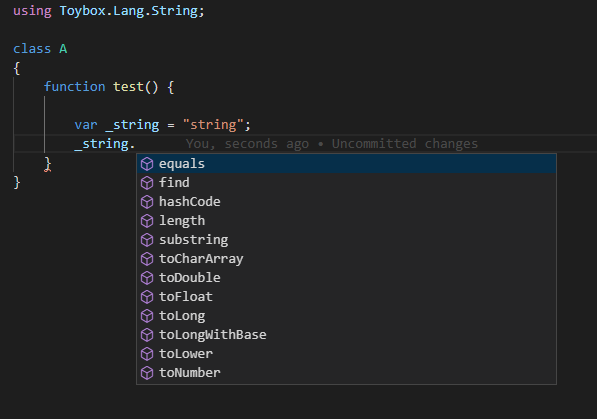
\includegraphics[scale=0.85]{images/autocomplete_example}
	\caption{ukázka automatického našeptávání kódu na proměnné typy string}
	\label{img:autocomplete_example}
\end{figure}

\begin{figure}[b!]
	\centering
	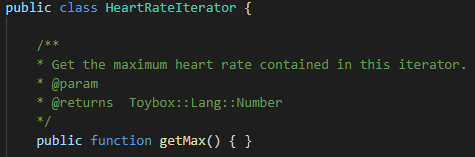
\includegraphics{images/comments}
	\caption{komentář nad funkcí obsahující stručný popis, parametry funkce a návratový typ}
	\label{img:comments}
\end{figure}

\section{Popis funkcí a proměnných Toyboxu}
Rozšíření dokáže při našeptávání jednotlivých částí Toyboxu zobrazit jejich název, druh a popis. A právě k jejich popisu bylo využito komentářů, která každá funkce a proměnná obsahuje. Tyto komentáře vznikly při generování Toyboxu a kromě popisu mají mnoho dalších účelů popsaných výše(např. našeptávání datového typu proměnné).
Na obrázku \ref{img:description} lze vidět popis funkce registerSensorDataListener() z modulu Toybox.Sensor. Součástí popisu je:

\begin{enumerate}
\item návratový typ funkce
\item název funkce
\item popis funkce
\item jednotlivé parametry společně s jejich datovým typem
\end{enumerate}

\begin{figure}[tbh!]
	\centering
	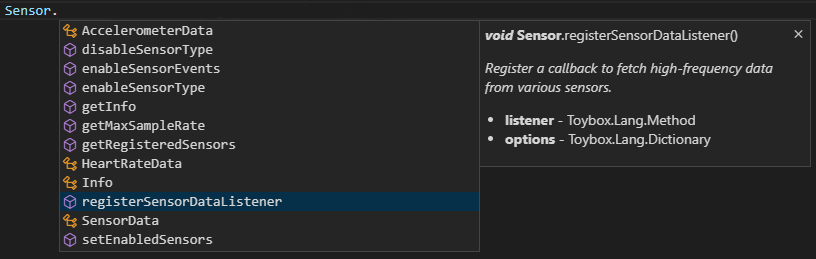
\includegraphics[width=\textwidth,scale=1]{images/description}
	\caption{popis funkce registerSensorDataListener() z modulu Toybox.Sensor.}
	\label{img:description}
\end{figure}


\section{Nedostatky rozšíření}
Při implementaci automatického našeptávání byl detekován problém, kvůli kterému není možné provést volání více funkcí po sobě na jednom řádku. Uveďme si příklad, kdy máme proměnnou typu \textbf{String}, v níž je uloženo číslo. Hodnotu v této proměnné budeme chtít převést na typ Integer, čili zavolat metodu \textit{toNumber()}, a poté bezprostředně po volání \textit{toNumber()} zavolat další metodu. Zde nastává problém, kdy rozšíření, jako další vstup neočekává možné volání funkce \ref{img:autocomplete_errormessage}. Jádrem tohoto problému je, že poskytnutá bezkontextová gramatika popisující jazyk není stoprocentně přesná. A právě kvůli těmto "nepřesnostem" je možné při implementaci narazit na podobné komplikace. V průběhu vývoje zatím nebyly registrovány další problémy způsobené gramatikou.

\begin{figure}[tbh!]
	\centering
	
\includegraphics[scale=1]{images/autocomplete_error}
	\caption{nedostatek rozšíření}
	\label{img:autocomplete_error}
\end{figure}

\begin{figure}[tbh!]
	\centering
	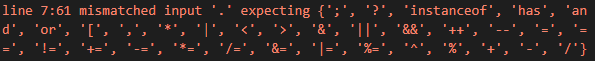
\includegraphics[scale=0.8]{images/autocomplete_errormessage}
	\caption{chybová hláška z error listeneru}
	\label{img:autocomplete_errormessage}
\end{figure}
\endinput
\chapter{Testování výsledného řešení}
Testování probíhá napříč mnoha fragmenty kódu.\\
Lorem ipsum dolor sit amet, consectetuer adipiscing elit. Aliquam erat volutpat. Etiam dui
sem, fermentum vitae, sagittis id, malesuada in, quam. Donec ipsum massa, ullamcorper in,
auctor et, scelerisque sed, est. Vivamus porttitor turpis ac leo. Sed ac dolor sit amet purus
malesuada congue. Maecenas aliquet accumsan leo. Etiam posuere lacus quis dolor. Curabitur
sagittis hendrerit ante. Duis condimentum augue id magna semper rutrum. Mauris dolor felis,
sagittis at, luctus sed, aliquam non, tellus. Integer vulputate sem a nibh rutrum consequat. Duis
pulvinar. Duis viverra diam non justo. Aenean vel massa quis mauris vehicula lacinia.
Fusce nibh. Sed ut perspiciatis unde omnis iste natus error sit voluptatem accusantium
doloremque laudantium, totam rem aperiam, eaque ipsa quae ab illo inventore veritatis et quasi
architecto beatae vitae dicta sunt explicabo. Quis autem vel eum iure reprehenderit qui in
ea voluptate velit esse quam nihil molestiae consequatur, vel illum qui dolorem eum fugiat
quo voluptas nulla pariatur? Etiam ligula pede, sagittis quis, interdum ultricies, scelerisque eu.
Maecenas sollicitudin. Cras pede libero, dapibus nec, pretium sit amet, tempor quis. Integer
vulputate sem a nibh rutrum consequat. Pellentesque sapien. Pellentesque arcu. Suspendisse
nisl. Fusce consectetuer risus a nunc. Etiam dui sem, fermentum vitae, sagittis id, malesuada
in, quam. Cum sociis natoque penatibus et magnis dis parturient montes, nascetur ridiculus
mus. Nam quis nulla. Nulla non lectus sed nisl molestie malesuada. Duis viverra diam non justo.
Sed ac dolor sit amet purus malesuada congue. Aenean id metus id velit ullamcorper pulvinar.
Aliquam ornare wisi eu metus. Neque porro quisquam est, qui dolorem ipsum quia dolor sit
amet, consectetur, adipisci velit, sed quia non numquam eius modi tempora incidunt ut labore
et dolore magnam aliquam quaerat voluptatem.
23
\chapter{Závěr}
Cílem této bakalářské práce bylo nastudovat jazyk Monkey C, nástroj ANTLR, díky kterému jsme schopni analyzovat a parsovat formální jazyky, a s jeho pomocí vytvořit parser jazyka Monkey C, jenž byl následně použit k analyzování kódu. 
\\
V úvodní části této práce se hovoří o tom, jak znatelně malé zastoupení má jazyk Monkey C na trhu s rozšířeními pro VS Code, vzhledem k ostatním programovacím jazykům. Tato skutečnost byla také jeden z hlavních důvodů, které vedly k tvorbě vlastního řešení. Dále byl v kapitole \ref{2Chapter} představen a popsán jazyk Monkey C, který je určen k vývoji aplikací a rozšíření pro zařízení Garmin, byly posány druhy aplikací, které je možné v Monkey C vyvíjet. Závěrem této kapitoly bylo porovnání Monkey C s ostatními moderními programovacími jazyky. Při vývoji rozšíření a následném testování jsem došel k závěru, že jazyk Monkey C má s ostatními, jako Python či Java mnoho společného. 
\\
Hlavním výsledkem práce je rozšíření pro VS Code, které uživateli napomáhá s psaním Monkey C kódu. Návrhem a implementací se zabývala kapitola \ref{5Chapter}. Byly zde popsány všechny důležité komponenty, jako providery pro našeptávání kódu, třída \textit{extension.ts}, ve které jsou providery implementovány, dále třída \textit{documentHandler.ts}, která obsahuje Mapy pro sémantickou analýzu a další podpůrné funkce pro parsování dokumentů, komunikaci s třídou \textit{Listener.ts}, která obsahuje callback funkce,e jenž odpovídají pravidlům gramatiky popsané v kapitole \ref{4Chapter}, atd... Během vývoje byly řešeny problému, jako jsou detekce modulů, funkcí, tříd a proměnných. Bylo řešeno našeptávání proměnných a funkcí, které jsou obsaženy ve třídě, pomocí klíčových slov \textbf{self.} a \textbf{me.}, které Monkey C využívá. Bylo řešeno parsování všech souborů, pokud se jich v pracovní složce nachází více. Dále byla řešena viditelnost mezi soubory, obarvení kódu pro jeho zpřehlednění, výpis chyb prostřednictvím ErrorListeneru, detekování datového typu proměnné pomocí komentáře, jenž je její součástí, atd... Součástí práce je i vygenerovaný modul Toybox, obsahující všechny potřebné třídy a funkce. Rozšíření bylo testováno na ukázkových kódech z oficiálního Connect IQ SDK.
\\
V této práci jsem uplatnil mnoho znalostí napříč různými jazyky. Využil jsem znalost jazyka JavaScript, jenž má prakticky totožnou syntax s Typescriptem. Dále jsem využil znalosti objektově orientovaného programování, které byly velmi užitečné při vývoji všech podpůrných tříd použitých ve finální aplikaci.\\
Díky této práci jsem měl také možnost rozšířit své znalosti o práci s jazykem Typescript. Dále jsem měl možnost pracovat s nástrojem ANTLR, který mě umožnil nahlédnout do problematiky překladačů a vývoji jazykových procesorů. Po dobu tvorby práce byl veškerý postup zaznamenáván pomocí verzovacího nástroje Git.
\\
Do budoucna by bylo možné třídu DocumentHandler rozšířit o tabulku symbolů, která by více zefektivnila sémantickou analýzu kódu, a tím pádem zvýšila účinnost a rychlost rozšíření. Dále by bylo vhodné nalézt efektivnější řešení pro generovaní Toybox modulu, jenž byl pro tuto práci vygenerován z html elementů obsažených v SDK. Jedním z možných řešení by bylo, kdyby společnost Garmin Ltd. \cite{GARMIN_OFFICIAL} tento modul v nějaké ucelené podobě zveřejnila.

\endinput

% Seznam literatury
\printbibliography[title={Literatura}, heading=bibintoc]

\end{document}
